\section{Künstlichen Sensordaten}
Im Projekt ist die Sensorenbox potentiell mit einem Accelerometer, Gyroskop, Lichtsensor, Magnetfeldsensor,
Temperatursensor und Geräuschsensor ausgestattet, sowie eine Antenne zur Erfassung von WLAN-Access-Points.
Mit CoppeliaSim ist es allerdings nur möglich Sensorwerte des Accelerometers, Gyroskops und Lichtsensors zu erfassen.
Aus diesem Grund werden die fehlenden Sensoren durch das Ausnutzen vereinfachter Modelle ergänzt.

\subsection{Magnetfeldsensor}
Magnetfeldsensoren messen das Magnetfeld auf Basis von Effekten die dadurch induziert werden, z. B. die Lorentzkraft oder der Hall-Effekt \cite{thompsonMEMS}.
Eine Anwendung dieses Sensors ist der Kompass.
Dieser richtet sich nach dem Magnetfeld der Erde aus und wird daher traditionell zur Navigation verwendet.
\newline
\newline
Das vereinfachte Modell des simulierten Magnetfeldsensors fungiert wie ein Kompass.
Die Ausgabe ist der relative Richtungsunterschied zum magnetischen Nordpol,
d. h. die Ausgabe ist relativ zur Ausrichtung des Objekts zum magnetischen Nordpol.
Dabei können starke magnetische Objekte in der Umgebung Einfluss auf den Sensor haben,
sodass sich der magnetische Nordpol für den simulierten Sensor ändern kann.
Die Ausgabewerte sind zwischen 0 und 359, d. h. 0 ist Norden, 90 Osten, 180 Süden und 270 Westen.
\newline
\newline
Es wird angenommen, dass der magnetische Nordpol der Erde weit genug weg ist,
sodass sich im Fabrikszenario die Richtung nur ändern kann, wenn die Ausrichtung des Objekts geändert wird.
Außerdem wird angenommen, dass sich die Ausrichtung des Objektes in einem Zyklus nicht ändert,
da Fließbandsysteme für gewöhnlich nicht rund sind, sondern Kante auf Kante aufeinander über gehen.
Allerdings wird für jeden Zyklus eine neue zufällige Ausrichtung zwischen 0 und 359 gewählt,
da das Objekt mit verschiedenen Ausrichtungen auf das Fließband gelegt werden könnte.
Zudem wird keine Interferenz der magnetischen Objekte angenommen.
Sollten sie sich überschneiden wird das Objekt mit dem meisten Einfluss gewählt.
\newline
\newline
Starke magnetische Objekte sind strategisch in der Umgebung des Fließbandsystems plaziert.
Ihre Stärke wird dabei durch die Einflussreichweite definiert, wobei der Einfluss quadratisch mit der Distanz abnimmt.
Ist der Einfluss bei 100\%, so wird für den magnetischen Nordpol die Position des Objekts angenommen.
Wenn der Einfluss geringer ist, dann wird ein magnetischer Nordpol zwischen dem magnetischen Nordpol der Erde und des magnetischen Objektes Anteilweise gewählt.
Die magnetischen Objekte können unterschiedliche Einflussreichweiten haben.
\newline
\newline
Abbildung \ref{fig:magnetic_model} illustriert diese Situation.
Um die Ausrichtung des Objekts relativ zum magnetischen Nordpol der Erde bei 0 und dem Einfluss des magnetischen Objekts zu berechnen,
ist es nötig die Winkel zwischen dem magnetischen Nordpol der Erde und dem magnetischen Objekt, sowie den Winkel zum Objekt zu wissen.
Der Winkel $\beta$ vom magnetischen Nordpol der Erde zum Objekt $p_{o}$ ist bekannt.
Der Winkel $\gamma$ vom magnetischen Nordpol der Erde zum magnetischen Objekt $p_{m}$ wird aus dem Winkel $\alpha$ innerhalb des eigenen Quadranten
und Anzahl der Quadranten, gezählt im Uhrzeigersinn, zum Quadranten indem $p_{m}$ liegt addiert.
\begin{figure}[h!]
    \centering
    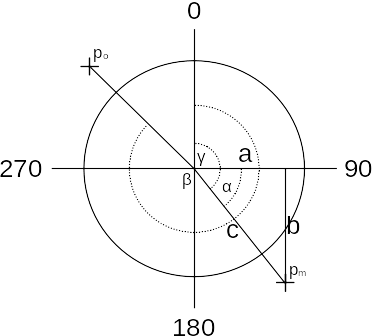
\includegraphics[width=0.7\linewidth]{images/magnetic_model.png}
    \caption{Berechnung der Ausrichtung des Objekts relativ zum magnetischen Objekt und magnetischen Nordpol.}
    \label{fig:magnetic_model}
\end{figure}
Je nach Quadrant können für $a$ und $b$ die $x$- bzw. $y$-Koordinate von $p_{m}$ gewählt werden.
Da der Einfluss des magnetischen Objekts $p_{m}$ abhängig von der Position des Objekts $p_{o}$,
müssen $a$ und $b$ dementsprechend transformiert werden.
Die Berechnung von $\alpha$ folgt dann Formel \ref{formular:magnetic_sensor_alpha}.
\begin{align}
    \label{formular:magnetic_sensor_alpha}
    \alpha = \arcsin (\frac{\abs(p_{o_a} - p_{m_a})}{\sqrt{(p_{o_a} - p_{m_a})^2 + (p_{o_b} - p_{m_b})^2}})
\end{align}
Mit den Winkeln $\gamma$ und $\beta$ kann dann das Koordinatensystem zum magnetischen Objekt hin rotiert werden,
sodass die Ausrichtung von $p_{o}$ zum beeinflussten magnetischen Nordpol aus Formel \ref{formular:magnetic_sensor_new_heading} berechnet werden kann.
\begin{align}
    \label{formular:magnetic_sensor_new_heading}
    \gamma^{\prime} = (\gamma + (360 - \beta))\ \%\ 360
\end{align}
Zu beachten ist schließlich der Einfluss $\eta$ abhänging von der Distanz das $p_{m}$ auf $p_{o}$ hat.
Formel \ref{formular:magnetic_sensor_influence} modelliert den Einfluss als quadratisch abfallende Funktion mit zunehmender Distanz $d$,
wobei der maximale Einfluss 1 ist und der minimale Einfluss 0.
\begin{align}
    \label{formular:magnetic_sensor_influence}
    \eta(d) = \min(0, 1 - \frac{d^2}{d_{\max}^2})
\end{align}
Der Einfluss wirkt sich proportional auf den Winkel von $p_{m}$ zum magnetischen Nordpol der Erde aus.
Dabei ist aber die Ausrichtung von $p_{m}$ zum magnetischen Nordpol der Erde zu beachten, denn beim Südpol ändert sich die Richtung des Magnetfeldes.
Formel \ref{formular:magnetic_sensor_end_result} zeigt die Berechnung von $\gamma^{\prime}$ abhänging von der Ausrichtung von $p_{m}$ zum magnetischen Nordpol der Erde,
wobei $d = \sqrt{(p_{o_a} - p_{m_a})^2 + (p_{o_b} - p_{m_b})^2}$.
\begin{align}
    \label{formular:magnetic_sensor_end_result}
    \gamma^{\prime}_L = (\gamma + (360(1 + \eta(d)) - \beta(1 - \eta(d))))\ \%\ 360 \\\nonumber
    \gamma^{\prime}_R = (\gamma + (360 - \beta(1 - \eta(d))))\ \%\ 360 \hspace{0.8cm}
\end{align}



\subsection{Temperatur}
\begin{itemize}
    \item Welchen Sensor spiegelt das wieder?
    \item Wie funktioniert das Modell?
    \item Was und Wie wurden Daten ergänzt?
\end{itemize}

\subsection{Lautstärke}
\begin{itemize}
    \item Welchen Sensor spiegelt das wieder?
    \item Wie funktioniert das Modell?
    \item Was und Wie wurden Daten ergänzt?
\end{itemize}

\subsection{WLAN Zugangspunkte}
\begin{itemize}
    \item Welchen Sensor spiegelt das wieder?
    \item Wie funktioniert das Modell?
    \item Was und Wie wurden Daten ergänzt?
\end{itemize}